This section describes the exploration of the software/hardware co-design space.
The software side includes partitioning the program, determining the number of threads and the specific source-level optimisations.
The hardware side is about finding out the best core composition that maximises performance for a given partitioning.

\begin{figure}[t]
 \centering
    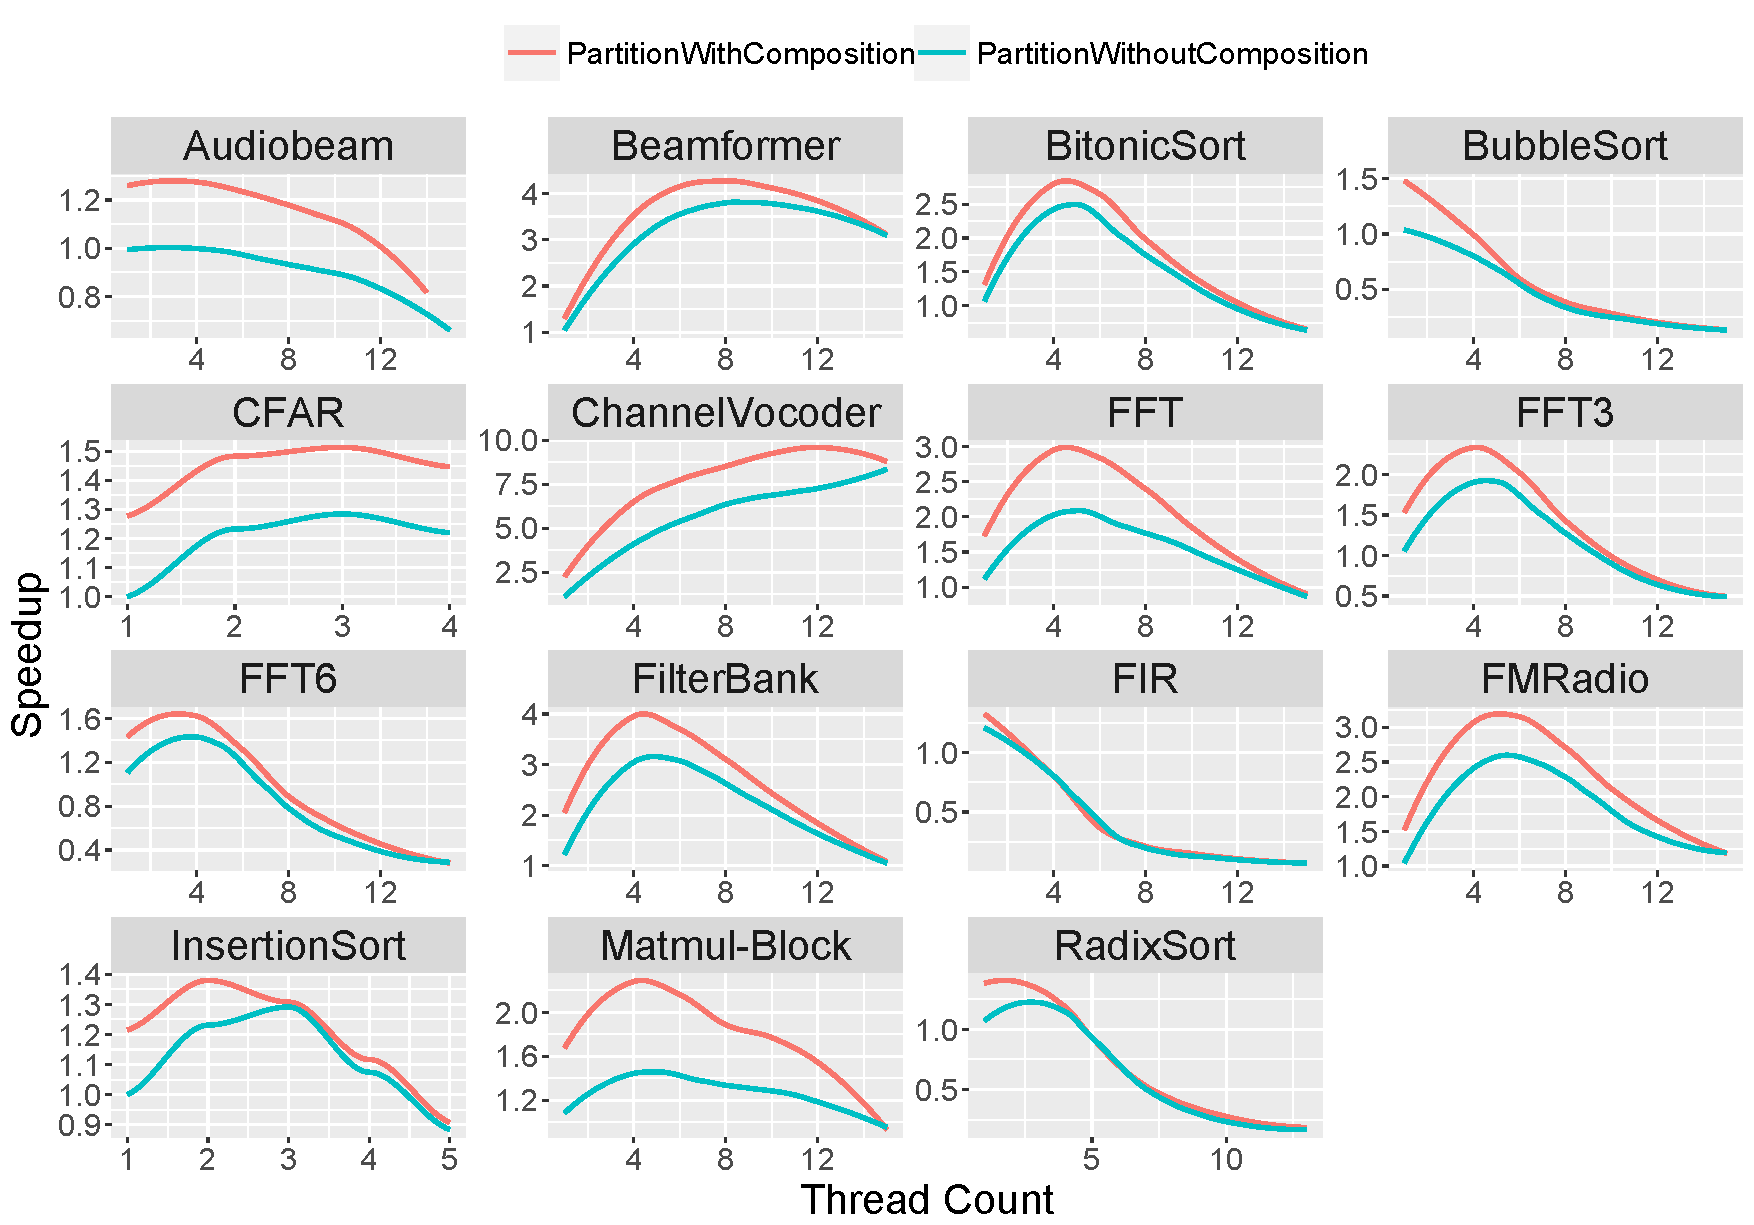
\includegraphics[width=1\textwidth]{streamit-paper/graphics/threadingmaybe5.pdf}
    \caption{Speedup obtained when increasing the number of threads with and without core composition. Baseline is single core single thread. Higher is better}\label{fig:threadtrend}  \vspace{-1em}

\end{figure}

\subsection{Thread Partitioning}

In this section, the term optimal number of threads defines the number of threads that results in the best performance for any given benchmark.
Thread partitioning is about deciding how many threads to create and how to partition filters into these threads.
To simplify this study, the default streaming partitioner is used to decide on how to allocate filters to threads which is based on simulated annealing~\cite{simulatedAnnealing1983}.

On the hardware side, two scenarios are considered: the ``without composition scenario'' where there is exactly one core per thread and the ``with composition scenario'' where each thread receives between 1 and 15 cores.
Figure~\ref{fig:threadtrend} plots how performance varies under both scenarios as a function of the number of threads.
In this figure, the ``with composition scenario`` uses points from the sample space that result in the fastest execution time for a given number of threads.
Once again, performance is measured by comparing the execution time of a design point to that of the single core/single thread as it represents the default configuration

Overall the optimal number of threads using core composition is very similar to the scenario without composition as both curves follow the same performance trends.
This is due to the fact that StreamIt is oriented towards task-level parallelism and thus, multithreading is a natural fit for performance improvements whilst core-composition may have less of an effect.
As both scenarios follow the same trends the optimal number of threads for a benchmark can be estimated independently from the hardware composition.
Also, since the number of cores in a composition is decided based on the amount of instruction level parallelism estimated in a thread, as will be explained in Section~\ref{sec:ml}, the thread count must be chosen before deciding on the number of cores that will be allocated to each thread.
The system can therefore proceed in two stages: first determine the optimal number of threads and then decide on a core composition.

Figure~\ref{fig:threadtrend} also shows that the performance of most benchmarks starts to deteriorate passed a certain number of threads making it critical to not over-allocate threads.
Since the optimal number of threads varies between benchmarks, there is no general thread count that can be applied to all of them.
By conducting a feature analysis of the set of applications, a model can be built to determine the optimal thread count for each of the benchmarks.
This procedure lends itself well to the use of machine learning.
Finally it is important to observe that executions without compositions always perform worse and thus it is essential to consider composing cores to get the optimal performance.


\subsection{Core Composition}

\begin{figure}[t]
  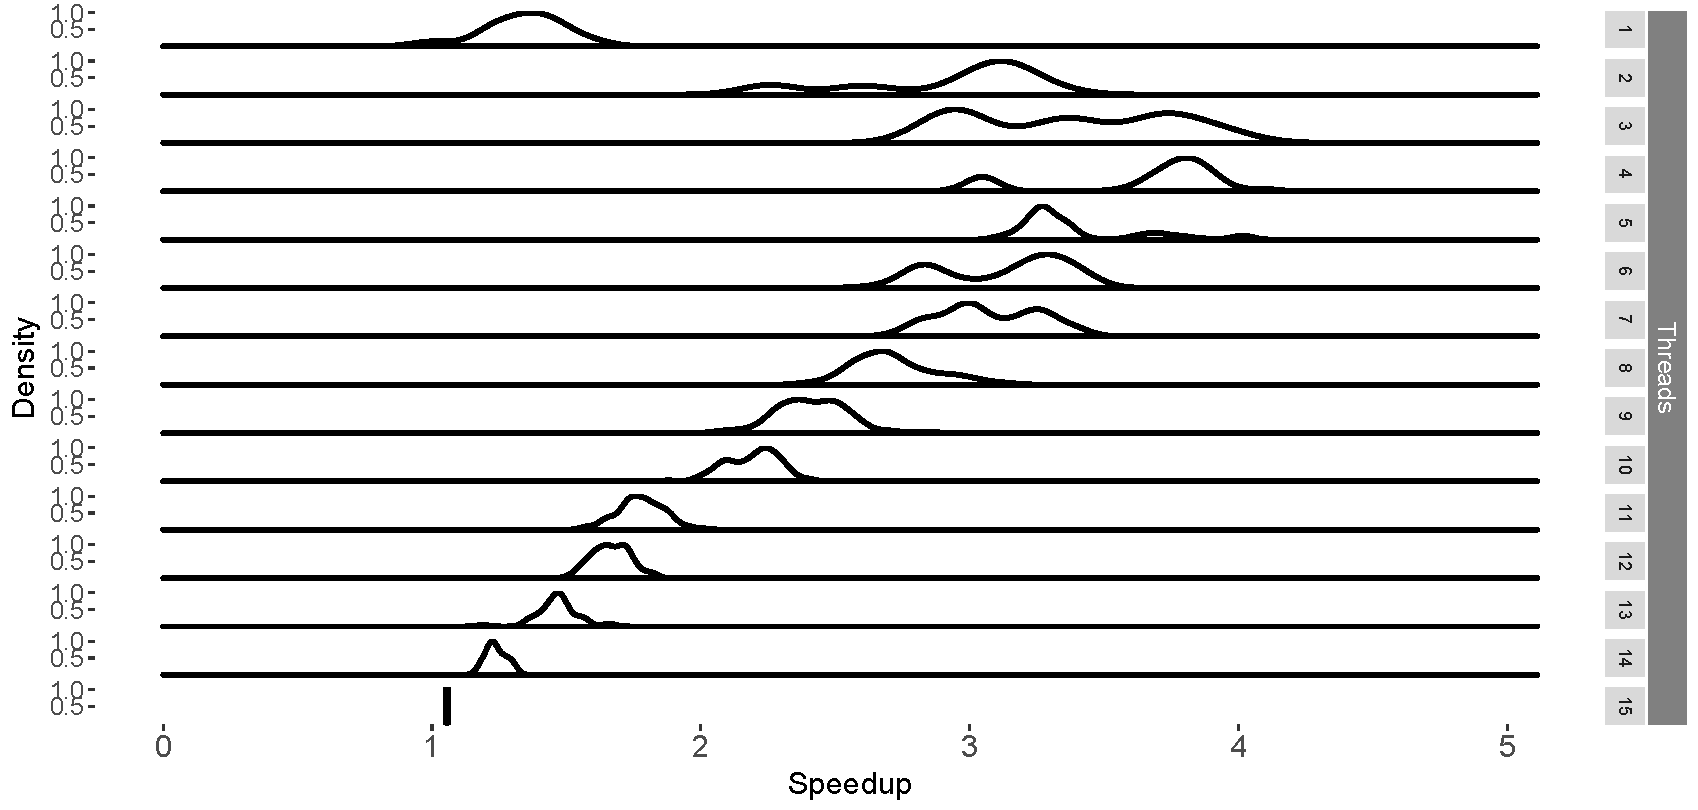
\includegraphics[width=1\textwidth]{streamit-paper/graphics/filterbank_tot2.pdf}
  \caption{Distribution of FilterBank performance when modifying the amount of threads and compositions. Speedup is obtained by comparing performance of configuration to single core, single thread.}\label{fig:fbtotal}
\end{figure}

Using core composition, the processor fuses a number of cores and associates them to a thread to increase its performance.
Whilst this flexibility is advantageous, choosing the right amount of cores for a given thread is difficult due to the large number of possible configurations~\cite{gulati2008multitaskingdmc}.

Figure~\ref{fig:fbtotal} shows how multi-threading and core compositions affect performance for the \bench{FilterBank} benchmark.
The curves represent the density distribution of speedups, compared to single core/single thread, for different core compositions as a function of the number of threads.
The right hand side Y-axis represents the number of threads present in the current version of the benchmark whilst the left Y-Axis represents the density normalised by the total number of points in the design space.
For each of the thread counts the benchmark is executed with 100 different core-compositions.
The density curve for thread 15 is a single point as there exists only a single composition, so a line is drawn to represent where that point lies.
Whilst only \bench{FilterBank} is shown here, a figure for each of the benchmarks was generated and can be found in the Appendix Figures \ref{chp:stream:at} through \ref{chp:stream:rt}

The width of each of the curves represents the influence of composition on the \bench{FilterBank}'s performance for a given number of threads.
For this benchmark, the impact of having core-composition enabled often leads to a 1.5x speedup compared to running only in multi-threaded mode; this can be seen for 1 to 4 threads.
Interestingly, as more threads are used, performance worsens, echoing the results shown in the previous section.
This is due to the fact that when the number of threads is increased, synchronisation between threads will increase whilst the potential number of cores which can be fused decreases.
In the case where the application does not feature highly parallel tasks, de-prioritising core compositions can negatively impact performance.
This signifies that for the benchmark \bench{FilterBank}, it is more important to compose cores with a small amount of threads rather than add more threads to the application.



\subsection{Impact of Loop Transformation}
Composing cores exploits instruction parallelism by running multiple EDGE blocks on a composition.
As physical cores in a core composition must communicate to submit block address predictions, and commit information to each other, having a small number of blocks will reduce the communication overhead.
Since physical cores can fetch more than a single block when the blocks are small, if the program being executed is comprised of mainly small blocks this will cause a composition to fetch very frequently.
Thus finding methods to increase the average size of the blocks can lead to reduced overhead which improves the core composition's ability to exploit instruction level parallelism (ILP).
One method of increasing the size of the blocks is through loop unrolling, and thus the impact of loop unrolling is studied on the benchmarks.

\begin{figure}[t]
  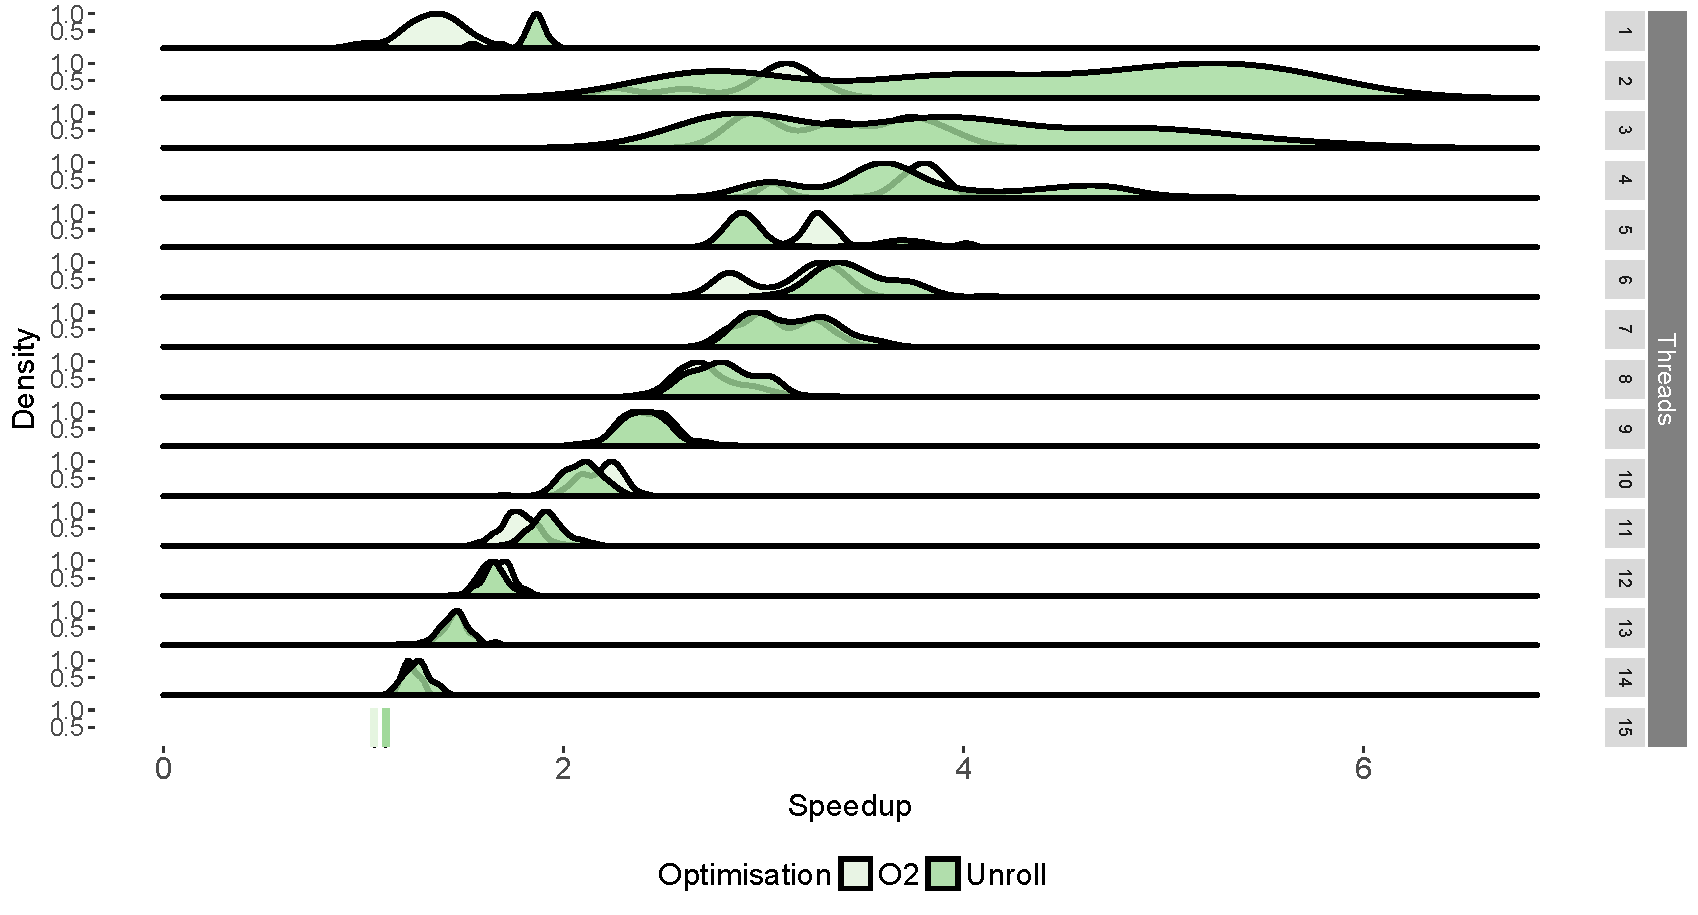
\includegraphics[width=1\textwidth]{streamit-paper/graphics/filterbank_unroll2.pdf}
  \vspace{-1em}
  \caption{Distribution of FilterBank performance when modifying the amount of threads, composition and unrolling factor. Speedup is obtained by comparing performance of configuration to single core, single thread without unrolling.}\label{fig:fbunroll}  \vspace{-1em}

\end{figure}

In this Chapter, unrolling is done at the source level via a flag passed to the StreamIt source-to-source compiler.
Given a number of times the loops must be unrolled, the StreamIt source-to-source compiler will generate the multi-threaded C++ code with the loops unrolled.
Figure~\ref{fig:fbunroll} presents an example of how loop unrolling affects performance on the \bench{FilterBank} benchmark.
The graph presents the same information as Figure~\ref{fig:fbtotal} but comparing O2 optimisations with O2 and Unrolling.
Figure~\ref{fig:fbunroll} shows that unrolling loops for \bench{FilterBank} can improve performance by up to 1.42x compared to the fastest non-unrolled version.
%Another observation is that the best speedups for each of the threaded versions when unrolling does not follow the same trend seen in Figure~\ref{fig:threadtrend}.
%The leftmost curve performance peaks at two threads whereas the rightmost peaks at 3 compared to 4 in the non-unrolled version.

\begin{figure}[t]
  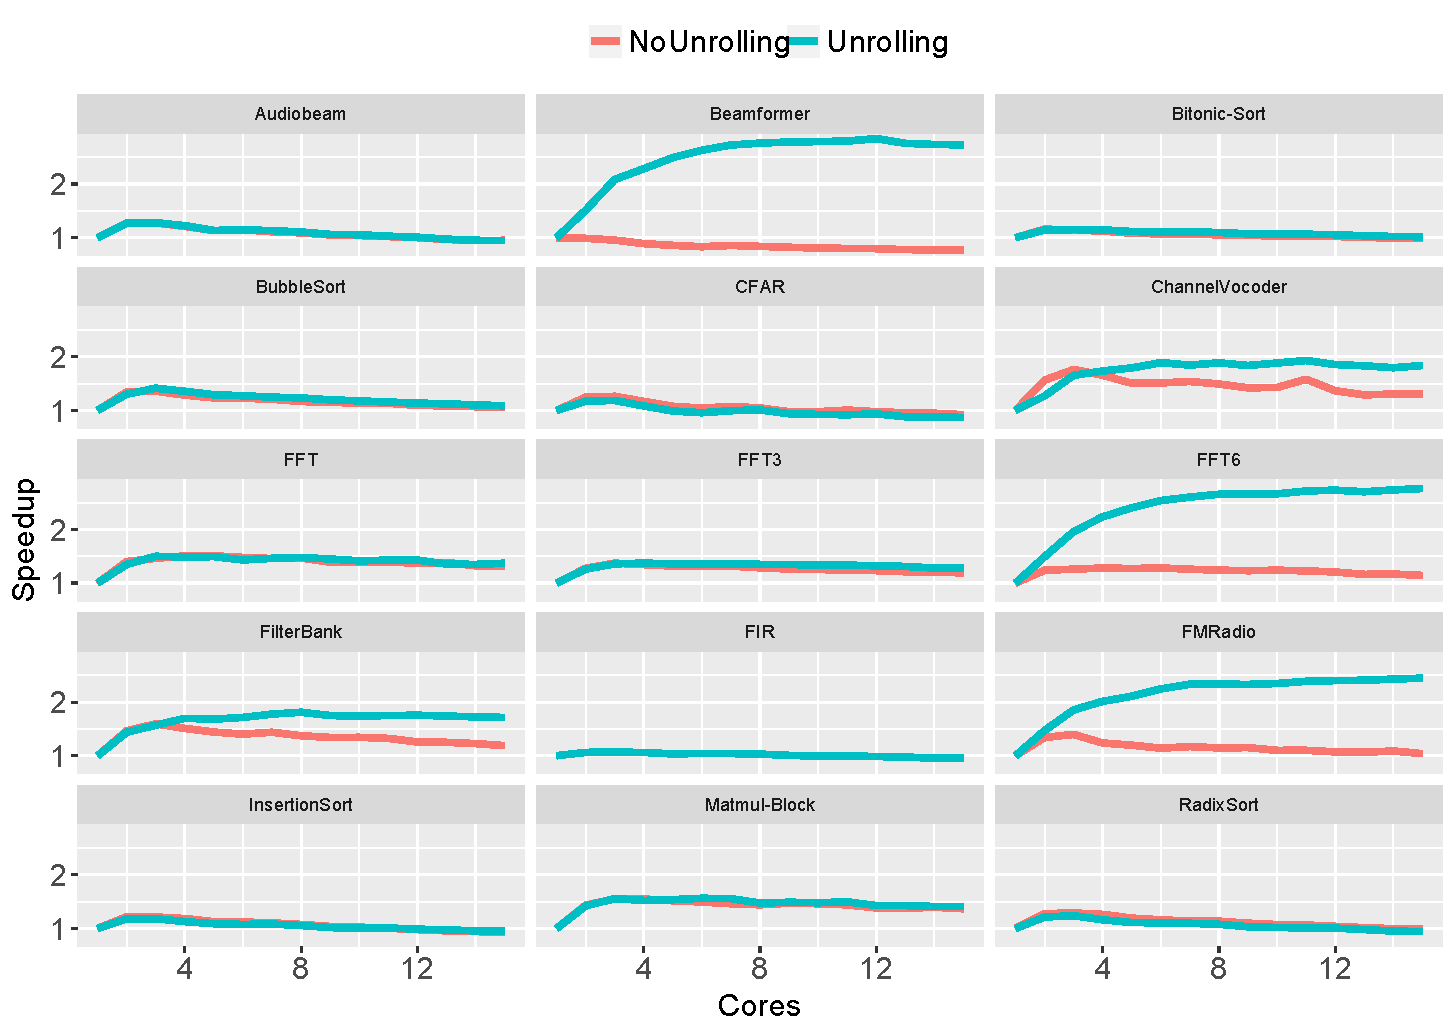
\includegraphics[width=1\textwidth]{streamit-paper/graphics/unroll_speed_bars2.pdf}
  \vspace{-1em}
  \caption{Effect of unrolling on performance via core-composition on the single-threaded versions of each benchmarks. The baseline is single core single thread.}\label{fig:unroll_summary}
  \vspace{-1em}
\end{figure}

Figure~\ref{fig:unroll_summary} shows how unrolling affects the amount of speedup obtained by running each of the StreamIt benchmarks on a single thread using different number of cores in the composition.
The X axis represents the number of cores in the composition, ranging from single core to 15 whilst the Y axis compares the execution time in number of cycles for the benchmark using a single core vs. a given core composition.
The colours of the lines represent with and without unrolling.
As can be seen, five benchmarks benefit from unrolling, these are \bench{Beamformer}, \bench{ChannelVocoder}, \bench{FFT6}, \bench{FilterBank} and \bench{FMRadio}. 
Figure~\ref{fig:unroll_bars} complements Figure~\ref{fig:unroll_summary} by showing the speedup obtained by unrolling loops when executing the benchmark on a single core.
On average, the information shown in Figure~\ref{fig:unroll_bars} and Figure~\ref{fig:unroll_summary} coincide: benchmarks that don't scale see no difference in performance when loop unrolling is called.

\begin{figure}[t]
  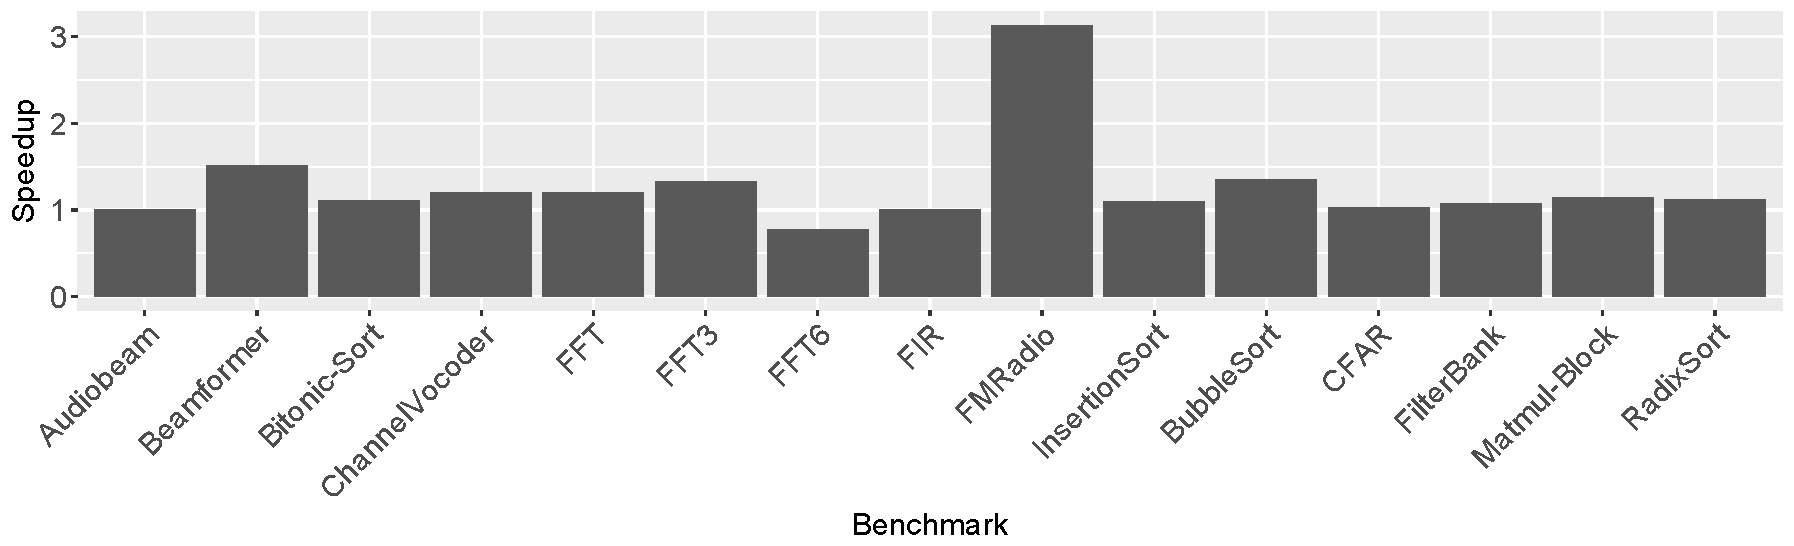
\includegraphics[width=1\textwidth]{streamit-paper/graphics/unroll_speed_bars.pdf}
   \vspace{-2em}
 \caption{Speedup obtained when executing on a single core with and without loop unrolling. Higher is better.}\label{fig:unroll_bars}
\vspace{-0.5em}
  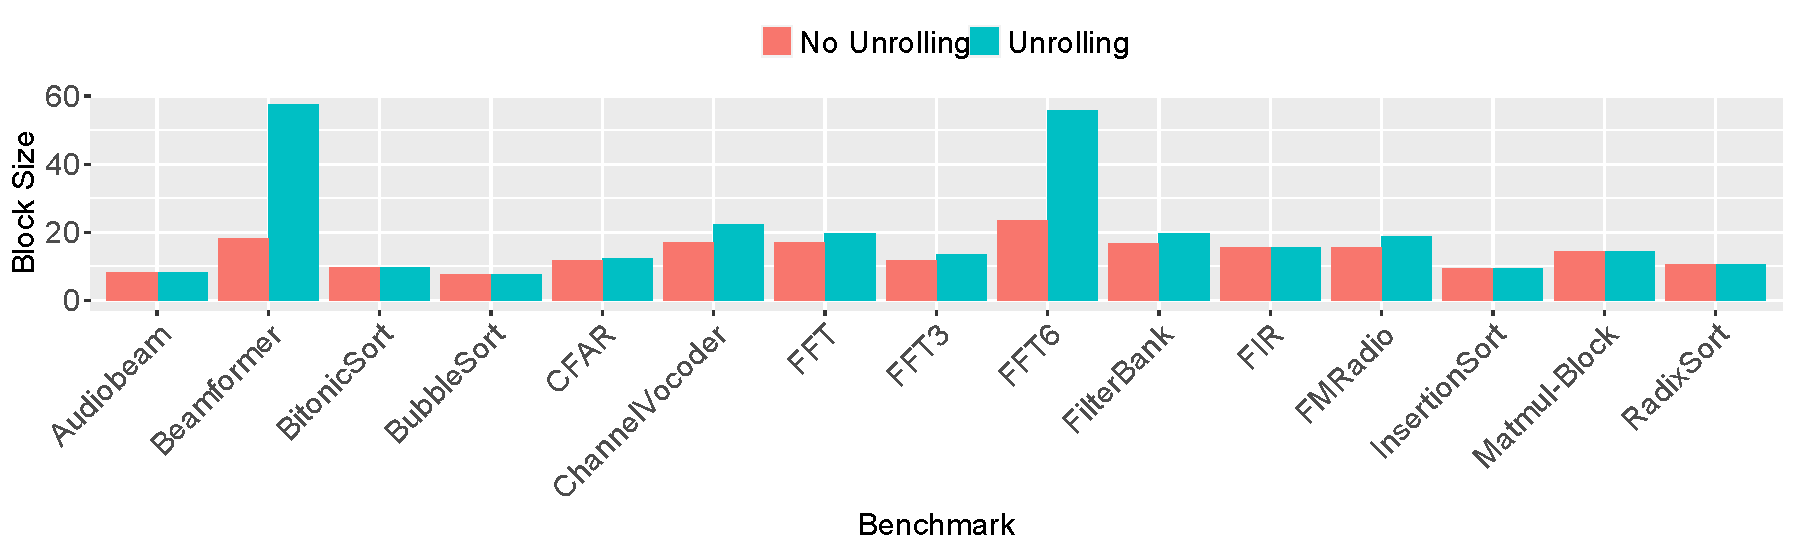
\includegraphics[width=1\textwidth]{streamit-paper/graphics/unrolling_size.pdf}  \vspace{-2em}

  \caption{Average size (in instructions) of blocks executed with and without unrolling for each benchmark .}\label{fig:unroll_size}  \vspace{-1em}

\end{figure}
For the benchmarks that do not scale with unrolling; this is most certainly due to the for loops containing conditional statements which may keep the blocks size small.
When a loop that holds multiple conditional statements is unrolled, conditional statements may not be fused into a single block; thus the block size does not change.
This is due to the fact that the compiler cannot generate multiple instruction predicates per block.
Benchmark \bench{FMRadio} sees a 3x improvement compared to the non-unrolled version, this is due to the fact that all the loops are fully unrolled, reducing the total number of instructions required to execute the task.
For the \bench{FFT6} benchmark, unrolling loops will actually cause the single-core version to be slower than its not unrolled version.
%I think this is due to a refreshing performance thing
This is due to the fact that for \bench{FFT6}, the source to source unrolling adds intermediate variables in the loop which increase the number of loads and stores.
Whilst it may be slower on a single core, as seen in Figure~\ref{fig:unroll_bars}, having a core-composition running the thread will still result in faster execution that without loop-unrolling.

Figure~\ref{fig:unroll_size} shows the influence of loop unrolling on the average size of an EDGE block for each of the benchmarks.
The size represents the number of instructions executed in each of the blocks.
The data for \bench{Beamformer} and \bench{FFT6} in Figure~\ref{fig:unroll_size} corroborate the idea that larger block sizes results in better performance when composing cores.
For these benchmarks, unrolling increases the average size of the block by at least 3x, which in turn improves the performance of larger compositions as seen in Figure~\ref{fig:unroll_summary}.
Benchmarks \bench{ChannelVocoder}, \bench{FilterBank} and \bench{FMRadio} also see an increase in block size yet it is not as important and averages out at a 1.22x increase.
That said, even a small increase improves the ability of using core composition more efficiently.

Overall, this section has shown that unrolling can improve performance by increasing the size of blocks which helps improve the efficiency of core-compositions.

%\begin{landscape}
\begin{figure}[t]%\hspace{-1em}
    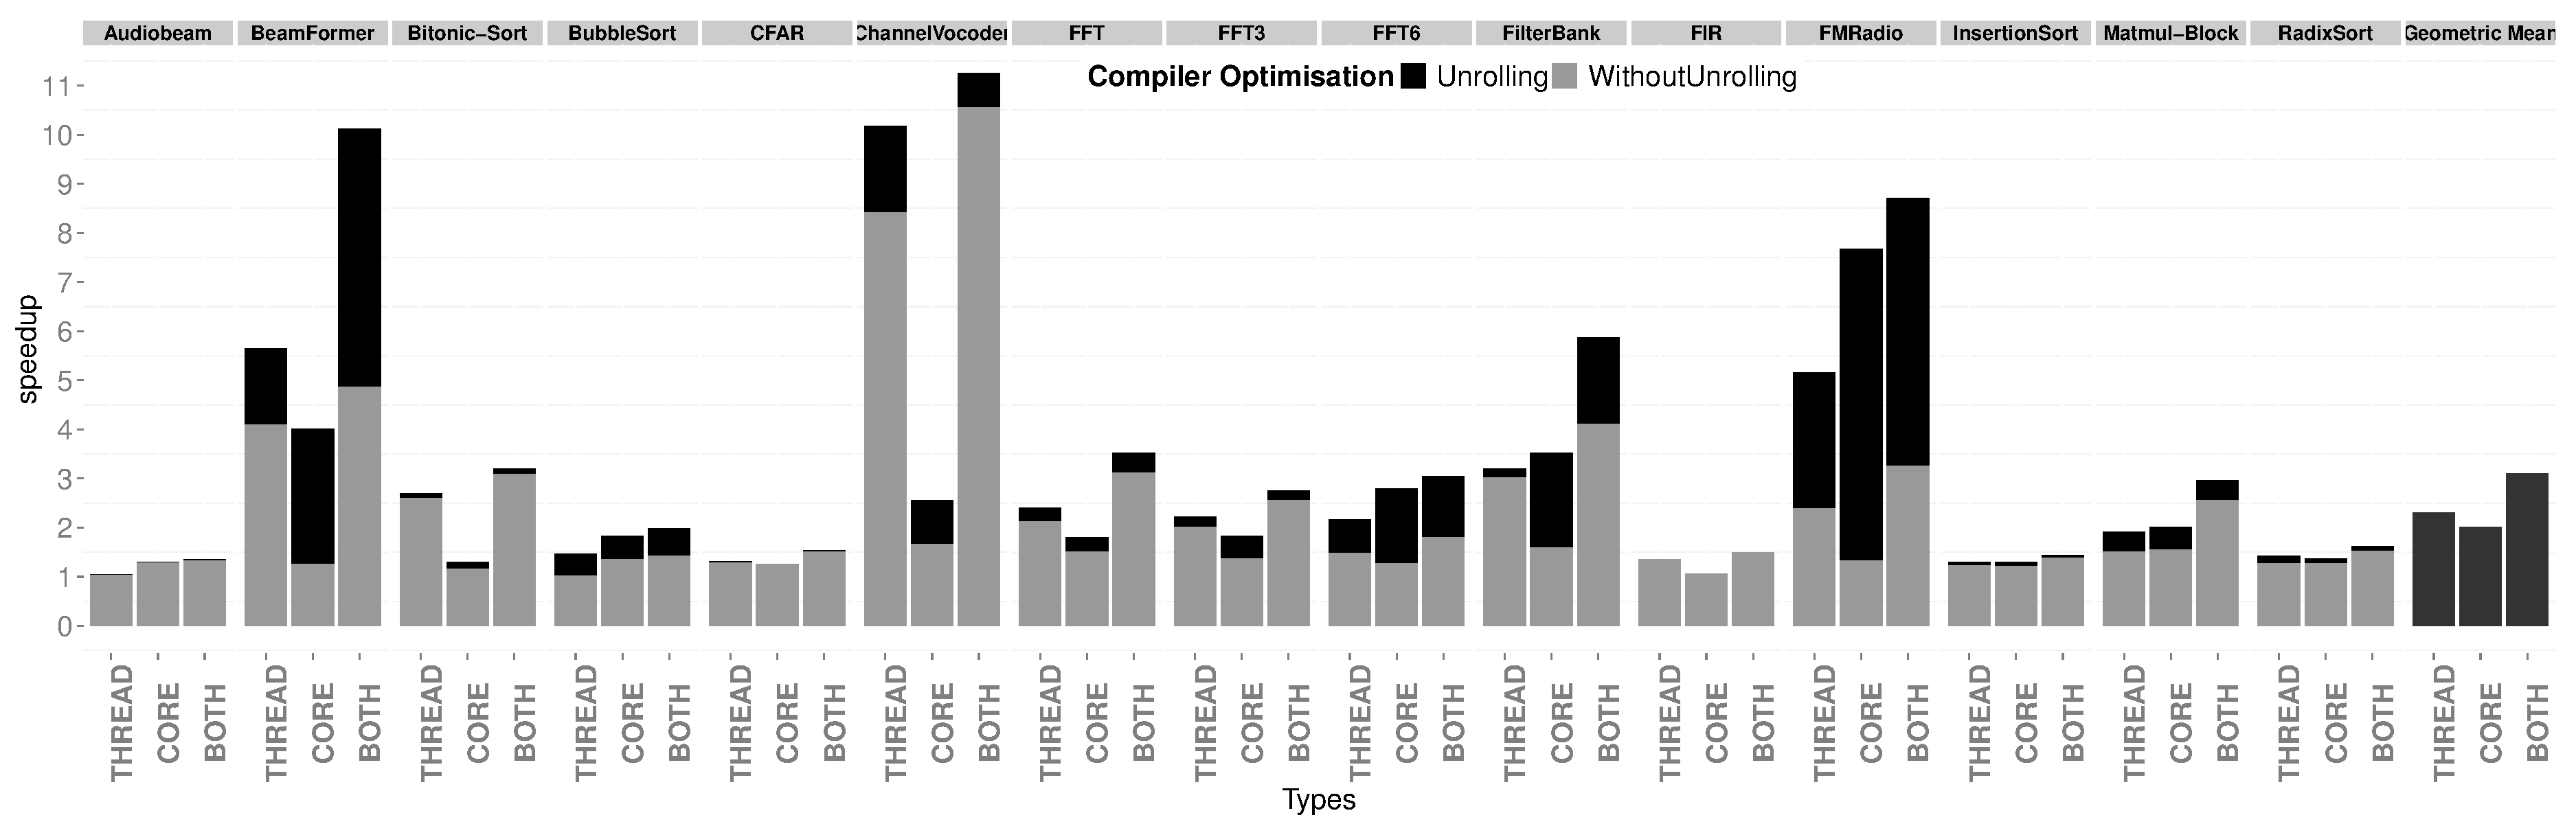
\includegraphics[width=1\linewidth,keepaspectratio]{streamit-paper/graphics/threadcompbench.pdf}
    \caption{Speedup obtained by choosing best core composition, best
      thread number and the combination of both optimisations. The baseline for the speedup measurement is single core, single thread execution using O2 compiler optimisations. Higher
      is better.}\label{fig:overviewhist}
\end{figure}
\subsection{Co-Design Space Analysis}


This section  presents the results of the entire co-design space exploration.
Figure~\ref{fig:overviewhist} characterises how much of a performance increase, over a baseline of a single-core single-thread with O2 optimisations, can be obtained with and without unrolling.
For each benchmark, the \textit{THREAD} bar represents the maximal speedup obtained by dividing the program into threads and assigning one core per thread.
The \textit{CORE} bar represents the best speedup when the benchmark is executed on a single thread and fuse all cores.
\textit{BOTH} represents the best speedup obtained for each benchmark using a combination of \textit{THREAD} and \textit{CORE}.
Finally, for each benchmark, the results are obtained for both an unrolled and not unrolled version to compare how the compiler optimisation affects performance.
Figure~\ref{fig:overviewhist} shows that when loops are not unrolled, composing cores will not greatly improve performance.
This is due to the fact that the amount of ILP found in filters without the unrolling is too little for there to be any benefit of composing cores.

In the scenario where there are no specific optimisations for composition, multithreading will be the main source of performance.
This can be seen when studying the average (geometric mean),without unrolling.
Finding the optimal number of threads gives a speedup of 1.92 compared to 1.33 when using only core composition, which is an improvement of 44\%.
This changes when taking unrolling into account as the core compositions can be used more efficiently.
In this case, the speedup obtained from composing cores without multithreading is only 13\% worse than using only threads.
For the \bench{FMRadio} benchmark, unrolling makes using only core-composition better than using multi-threads without core composition.
This information corroborates with the data seen in Figure~\ref{fig:unroll_summary}; it presents a unique case where the effect of core composition is important enough to change the dominant performance enhancer.
The performance increase obtained via the source-level loop unrolling via the compiler demonstrates that some modifications to the code must be done to ensure optimal use of the dynamic multicore processor.
%Thus loop unrolling demonstrates that the StreamIt programs must be modified to take advantage of the core composition.

Overall the results show that for these applications, multithreading leads to more performance gains than using core composition.
This is natural as StreamIt applications are naturally geared towards thread level parallelism (TLP) as most programs have at least one SplitJoin as seen in the Table~\ref{tab:instancefilt} which gives the number of split-joins per benchmark.
Benchmarks with SplitJoins will naturally benefit from splitting the program into threads~\cite{thiesStreamit2010}.
%Make sure this is 100% true but as far as I remember this is the case
Those that do not feature SplitJoins can still be parallelised by splitting a Pipeline into multiple parts.
For example, benchmark \bench{FIR} features no SplitJoins, yet splitting the Pipeline in 2 will result in a 1.40x speedup.
However, it is important to note that whilst finding the optimal thread mapping may result in higher performance improvements than finding the optimal composition for a single thread, the best performance is always obtained through a combination of both techniques.
For cases such as \bench{BeamFormer} the optimal pairing results in a 1.8x speedup compared to simply finding the best multithreaded version.
On average, the optimal combination leads to a 1.5x performance increase compared to only multithreading.

%\end{landscape}
\subsection{Summary}
This section has demonstrated that each parameter has a large effect on the performance of the workload.
Regardless of using core composition, there exists an optimal number of threads for each benchmark.
Unrolling allows to exposing more opportunities for composition due to increased block sizes but there is a balance to strike between extracting large blocks and TLP.
Figure~\ref{fig:overviewhist} shows there is a 3x benefit overall by automating the partitioning of both the software (threads) and hardware (cores).

